\chapter{Study of the reconstruction of the \BdKstee invariant mass}
\chaptermark{Chapter4}
\label{chapter3}
%\addcontentsline{toc}{chapter}{Study of the reconstruction of the \BdKstee invariant mass}
The event reconstruction is a crucial part of the analysis of any decay. At \lhcb, the offline event reconstruction is made in two steps. The first step is executed by the software \brunel that performs subdetector and global reconstruction using pattern recognition for both Monte Carlo and real data. \brunel takes the detector information and reconstructs \textit{tracks} from the hits. The information for each \textit{track} is then stored for further analysis.\\
The second step, the one accessible and adjustable by every user, is executed by the \davinci physics and analysis framework. At the beginning of every event reconstruction \davinci builds lists of \textit{particles}. For each particle-type, such as electron or kaon, there are several lists ranging from very loose to very tight requirements on the \textit{tracks}. For each list, \davinci selects all the \textit{tracks} provided by \brunel that fulfil the list conditions and fully reconstructs them as \textit{particles}, quantities of physics with a four-momentum. In the course of this reconstruction the mass of the \textit{particle} is fixed to the particle-type's mass defined by the list.
%These \textit{particles} are made from the \textit{track} information provided by \brunel and are quantities of physics with a four-momentum. In the course of computing the \textit{particles} properties their masses are fixed to the value corresponding to the condition of the list, e.g. all particles in the list \textsc{SdtAllLooseKaons} have a mass of $493 \mevcc$.\\
From the lists of \textit{particles} \davinci reconstructs intermediate particles (e.g. \Kstarz from \Kp and \pim) and finally the entire \BdKstee decay. \davinci allows the user to choose the \textit{particle} lists and the algorithms that compute their properties, additionally to the way the \textit{particles} are being combined.\\ % einfuegen von bezug auf arbeit
\\
The greatest difficulty in reconstructing the \BdKstee decays is the measurement of the electron\footnote{Throughout this chapter electron stands for electrons and positrons if not mentioned otherwise.} energy. This difficulty arises from bremsstrahlung radiation and propagates to a vast degradation of the \Bd mass resolution. The effects occurring due to bremsstrahlung of the electrons and the means of limiting the loss in precision -- namely different event reconstruction tools implemented in the \davinci framework -- are presented in the following Section. \\
In Section \ref{sec:DiElectronMaker} the focus is put on the reconstruction on the invariant mass of the electron pair $M_{inv}(\epem)$.\\
\newpage
\section{Bremsstrahlung radiation}
\label{sec:bremsstrahlung}
When traversing the material of the detector charged particles undergo a probability of emitting bremsstrahlung. The cross-section for bremsstrahlung emission $\sigma_{bs}$ is anti-proportional to the square of the charged particle's mass $m$ \cite{WRLeo}.
\begin{equation}
 d\sigma_{bs} \propto \frac{e^2}{(mc^2)^2}
\end{equation}
Since the amount of material is low in \lhcb the probability of emitting bremsstrahlung photons is negligible for heavier particles, but very light particles such as electrons and positrons can lose a significant amount of energy through bremsstrahlung radiation. The amount of energy emitted through bremsstrahlung for muons $E_{bs}^{\mmu}$ for instance, is suppressed by a factor $40\ 000$ with respect to that of electrons $E_{bs}^{\electron}$.
\begin{equation}
\frac{E_{bs}^{\electron}}{E_{bs}^{\mmu}} = \frac{m_{\electron}^2}{m_{\mmu}^2} = 2.3 \cdot 10^{-5} 
\label{eq:evsmu}
\end{equation}
%At energies below a few \gev only electrons emit a significant amount of bremsstrahlung radiation in the \lhcb detector.\\
The radiated energy spectrum for the electrons from \BdKstee before the \lhcb magnet is shown in Figure \ref{fig:totalEnergyLossBrems}. The distribution was obtained by performing a Fast-Sim \cite{ananote} on Monte Carlo at simulation level under the assumption of complete screening \cite{pdg}.
\begin{figure}[ht]
  \begin{center}
    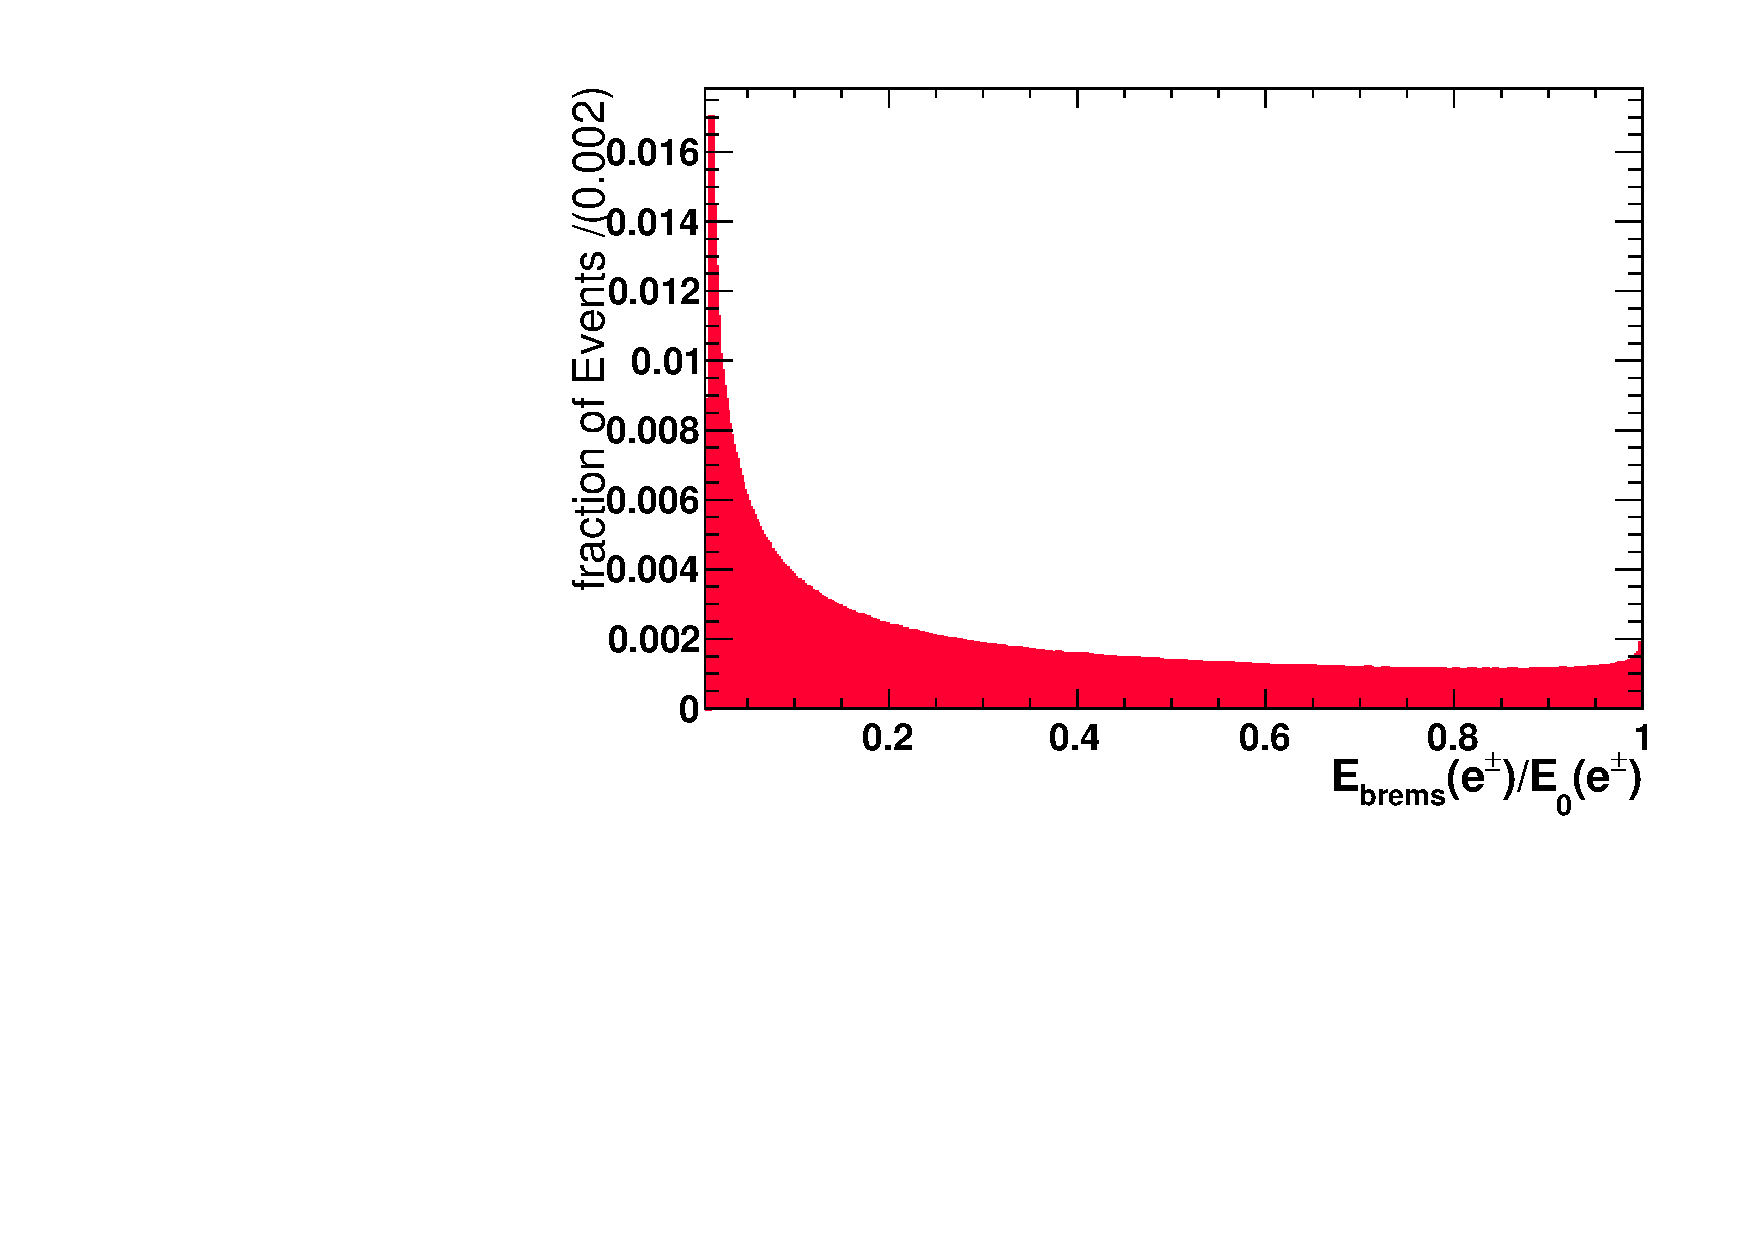
\includegraphics[width = 0.55\textwidth]{EnergyLossBrems.pdf}
    \end{center}
    	\vspace*{-0.8cm}
  \caption{\textit{Percentage of energy loss of electrons/positrons traversing the \lhcb detector before the magnet. $E_{brems}(\epm)$ denotes the energy radiated by the electron/ positron while $E_0(\epm)$ stands for the initial electron/positron energy. Distribution obtained by performing a Fast-Sim on Monte Carlo Data at simulation level under the assumption of complete screening.}}
  \label{fig:totalEnergyLossBrems}
\end{figure}

The bremsstrahlung radiation process is of statistical nature. Figure \ref{fig:totalEnergyLossBrems} shows the amount of radiated energy. It is therefore crucial to identify photons in the detector that have been emitted by electrons through bremsstrahlung radiation and add their four-momentum to the four-momentum of the electron track. The \Bd mass distribution without any kind of bremsstrahlung reconstruction can be seen in Figure \ref{fig:noBremReco}.
\newpage
\begin{figure}[ht]
  	\centering
    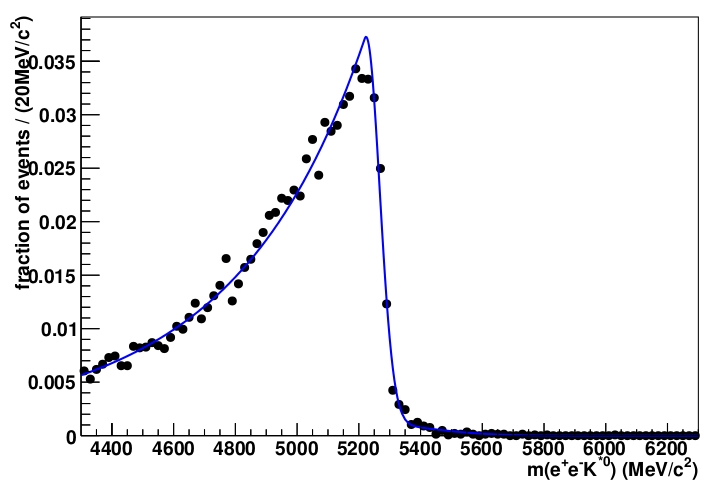
\includegraphics[width = 0.55 \textwidth]{oldBrem_noBremReco.jpg}
  \caption{\textit{The \Bd mass distribution of \BdKstee \lhcb Monte Carlo without any reconstruction of bremsstrahlungs photons.}}
  \label{fig:noBremReco}
\end{figure}

\subsection{Bremsstrahlung recovery}
\label{sec:bremsstrahlungrecovery}
If the emission of the bremsstrahlung happens before the magnet, the electron will be deflected from its initial trajectory by the magnetic field while the bremsstrahlung photon's momentum will not change, as shown in Figure \ref{fig:bremsstrahlung}. Thus, the electron and its photon will deposit their energies in different positions in the \ecal. To allow nonetheless for an assignment of the bremsstrahlung photon with its electron \textit{bremsstrahlung recovery algorithms} have been developed. These algorithms search for bremsstrahlung photon candidates in the \ecal and try to match them to the corresponding electron track.Two different bremsstrahlung recovery algorithms implemented in the \lhcb physics analysis framework will be presented in Sections \ref{sub:oldBrem} and \ref{sub:newBrem}.
\begin{figure}[ht]
\vspace*{-0.4cm}
  \begin{center}
    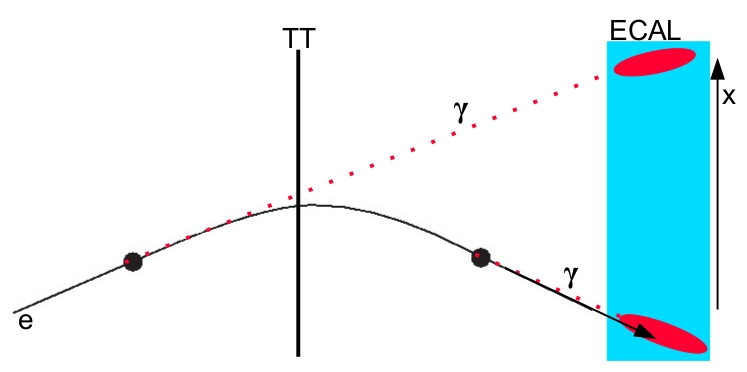
\includegraphics[width=0.6\textwidth]{BremReco.jpg}
  \end{center}
  \vspace*{-0.5cm}
  \caption{\textit{Schematic illustration of bremsstrahlung emission of electrons in the \lhcb detector.}}
  \label{fig:bremsstrahlung}
\end{figure}
If the emission of the bremsstrahlung happens after the magnet, the electron and its photon will deposit their energies in the same \ecal cells. Thus the photon energy is automatically added to the energy of its electron. \\


\subsubsection{Bremsstrahlung recovery algorithm in \davinci v29 }
\label{sub:oldBrem}
The first bremsstrahlung recovery tool was the standard algorithm implemented in all version of \davinci up to v29. An illustration of its methodology is shown in Figure \ref{fig:oldBremAdd}.
\begin{figure}[ht]
\vspace*{-0.5cm}
  \begin{center}
  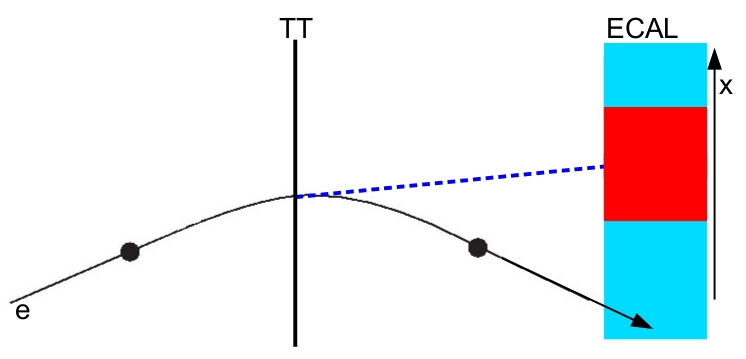
\includegraphics[width=0.6\textwidth]{oldBremAdder.jpg}
  \end{center}
  \vspace*{-0.5cm}
  \caption{\textit{Schematic illustration of the bremsstrahlung recovery algorithm \davinci v29. Black line: curve of the electron track. Dark blue dotted line: linear extrapolation of the electron track from its very first state to the \ecal. Clear blue dotted line: linear extrapolation of the electron track from its last state before the magnet to the \ecal. Red area in the \ecal: area from where photon candidates will be matched to the electron track.}}
  \label{fig:oldBremAdd}
\end{figure}
The algorithm starts with a \textit{particle} list of electrons and searches for reconstructed photon candidates coming from the electron tracks.
To predict the position of bremsstrahlung photon candidates in the \ecal, the algorithm linearly extrapolates the electron track from the \ttracker (last state before the magnet) to the \ecal. All neutral clusters in the \ecal whose barycentric positions match the position of the extrapolated electron track with a $\chi^2 < 300$ are accepted as bremsstrahlung photons. Their four-momentum is added to the four-momentum of the electron. Furthermore there is no limit of bremsstrahlung photon candidates that can be added to one electron.\\


\subsubsection{Bremsstrahlung recovery algorithm in \davinci v30}
\label{sub:newBrem}
The second bremsstrahlung recovery tool is implemented in \davinci v30. Its methodology is illustrated in Figure \ref{fig:newBremAdd}.
\begin{figure}[ht]
  \begin{center}
  \label{fig:newBremAdder}
  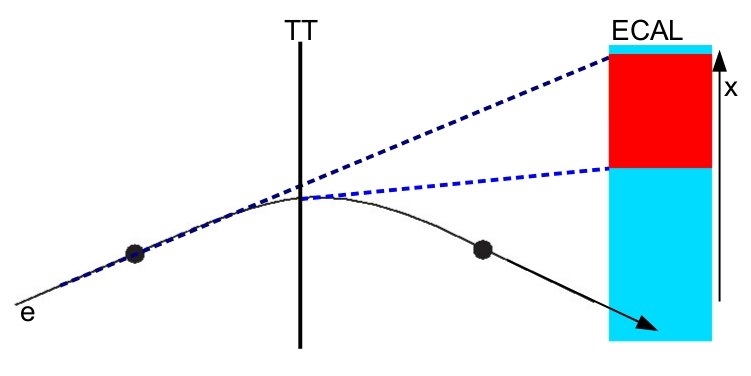
\includegraphics[width=0.6\textwidth]{newBremAdder.jpg}
  \end{center}
  \vspace{-0.8cm}
  \caption{\textit{Schematic illustration of the bremsstrahlung recovery algorithm \davinci v30. Black line: curve of the electron track. Dark blue dotted line: linear extrapolation of the electron track from its very first state to the \ecal. Clear blue dotted line: linear extrapolation of the electron track from its last state before the magnet to the \ecal. Red area in the \ecal: area from where photon candidates will be matched to the electron track.}}
  \label{fig:newBremAdd}
\end{figure}
For each \textit{particle} in the electron list two linear extrapolations of the track are computed, namely the extrapolation of the electron track from its very first state in the \velo to the \ecal and from its state in the \ttracker to the \ecal. Photon candidates must satisfy tighter conditions than for the algorithm in \davinci v29 \footnote{Photon candidates for the \davinci v30 bremsstrahlung recovery algorithm must satisfy the conditions of a PhotonID greater than $-0.5$ and a $p_T$ greater than $75 \mevc$.}.
The $x$ position of the photon candidates in the \ecal must lie between the $x$ positions of the two electron track extrapolations within $\pm 2 \sigma_{x}$. The $y$ position of the photon candidate in the \ecal must match the $y$ position of the electron track extrapolations within $\pm 2 \sigma_{y}$. The $\sigma_{x,y}$ denote the square root of the quadratic sum of the photon cluster spread with the error on the electron track extrapolations. \\



\subsection{The mechanism of double counting}
\label{sec:doublecounting}
Both bremsstrahlung recovery algorithms implemented in \davinci have the disadvantage of generating \textit{double counting}. Double counting occurs when one bremsstrahlung photon candidate can be associated to more than one electron track. This happens particularly often for the \BdKstee decay mode where the $e^+e^-$ invariant mass is very low, yielding small angles between the electron and the positron, as is illustrated in Figure \ref{fig:schemdc}. The distribution of double counting events depending on the $M_{inv}(e^+e^-)$ is shown in Figure \ref{fig:Minveedouble counting}. In the case of double counting the bremsstrahlung recovery algorithms add the photon's four momentum to both the electron's and the positron's four momentum. In the case of \BdKstee, these events will show a non-physically high $B^0$ mass and lead to a non-typical symmetric \Bd mass distribution that can be seen in Figure \ref{fig:oldBremAddernodcc}. 
\begin{figure}[ht]
\vspace*{-0.5cm}
  \begin{center}
  \label{fig:newBremAdder}
  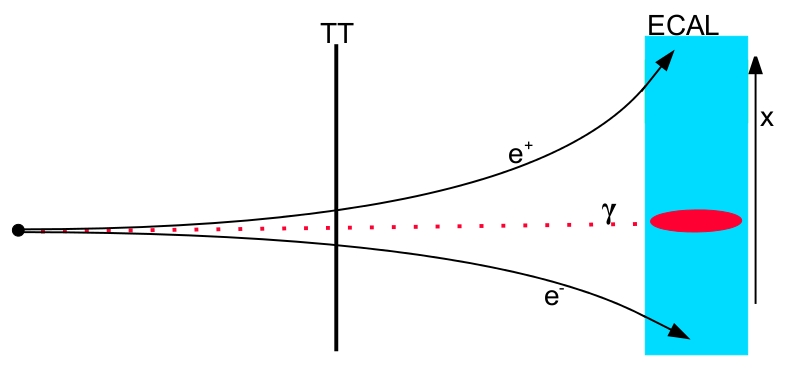
\includegraphics[width=0.6\textwidth]{doublecounting.jpg}
  \end{center}
  \vspace*{-0.5cm}
  \caption{\textit{Schematic illustration of the mechanism of double counting. Due to a very low $e^+e^-$ invariant mass the angle between the electron and the positron is so small that the photon can be associated to both.}}
  \label{fig:schemdc}
  \vspace*{-0.5cm}
\end{figure}

\begin{figure}[ht]
  \begin{center}
  \vspace*{-.6cm}
  \subfigure{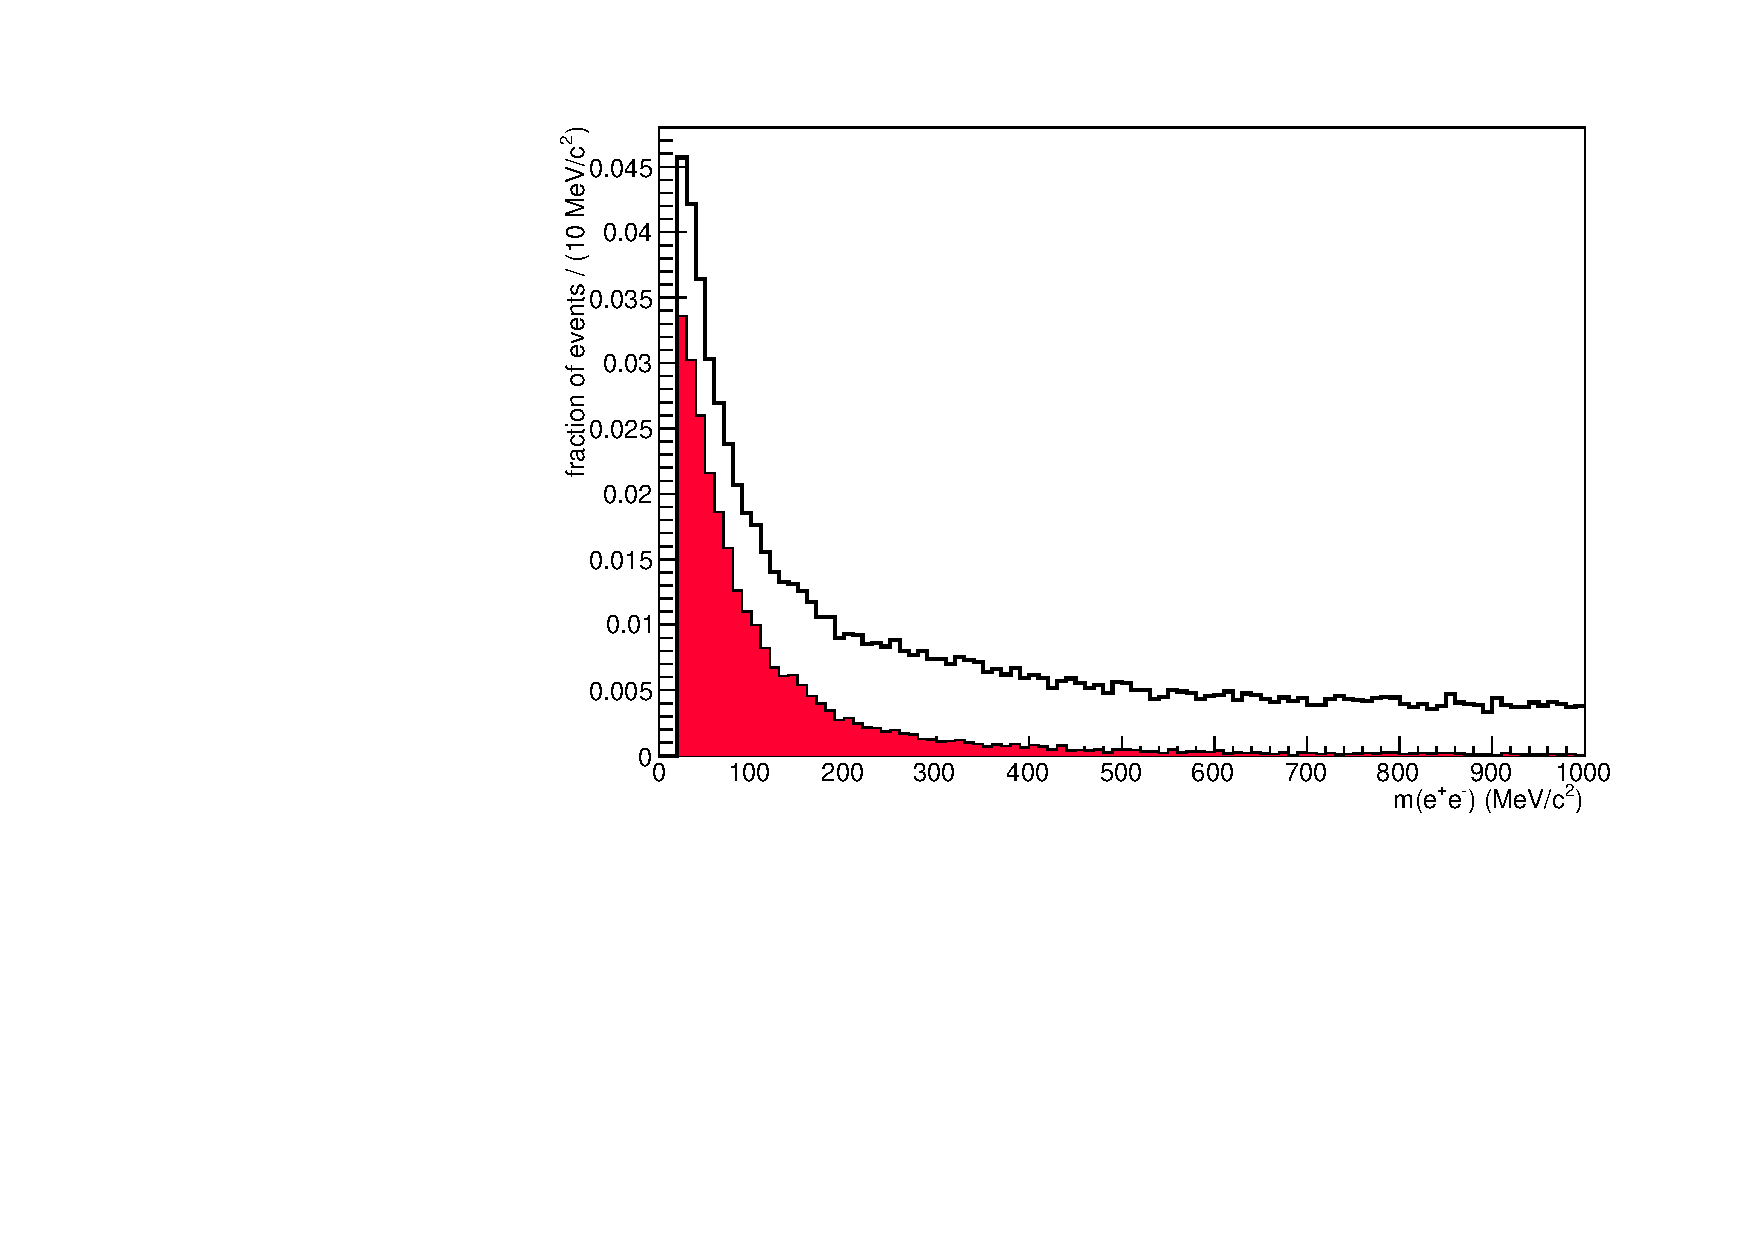
\includegraphics[width=0.48\textwidth]{dccats_Minvee_oldBrem.pdf}}
    \subfigure{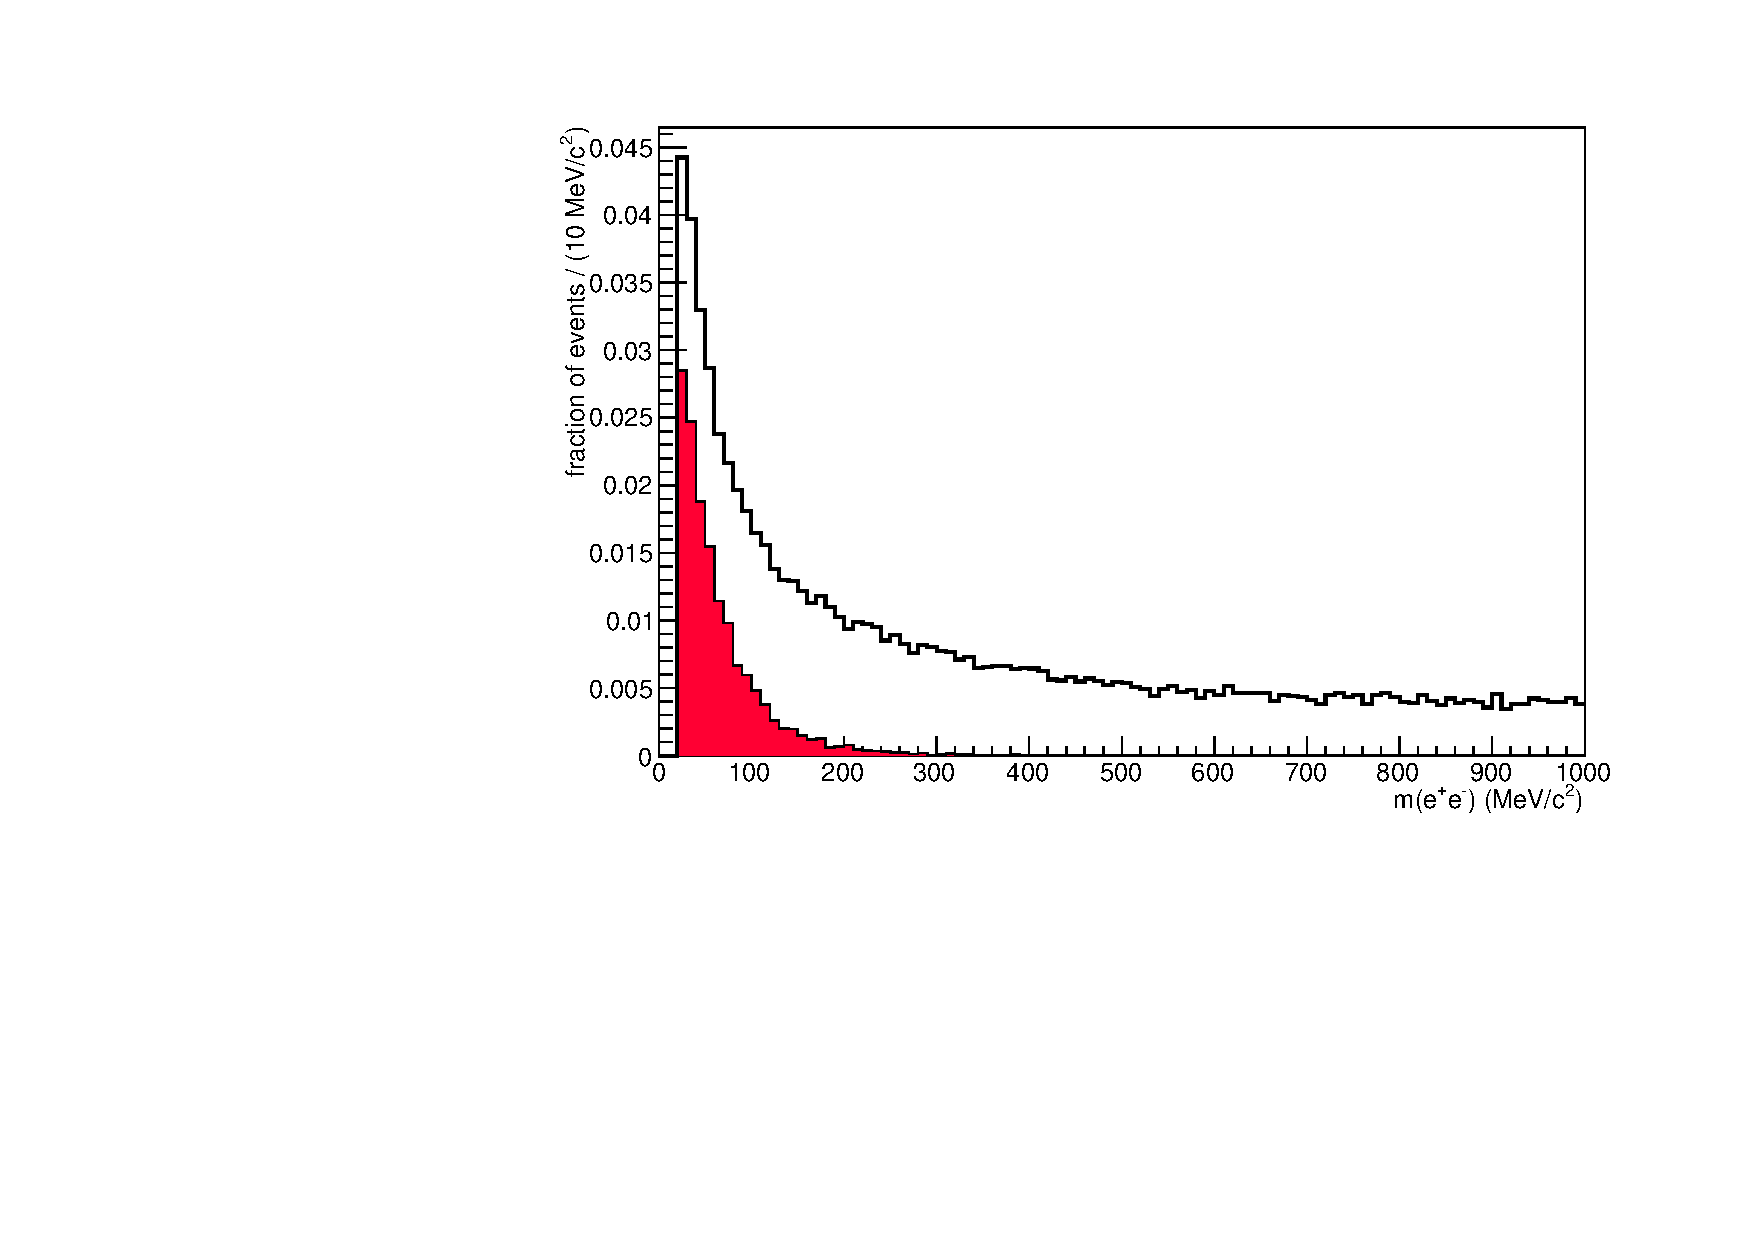
\includegraphics[width=0.48\textwidth]{dccats_Minvee_newBrem.pdf}}
  \vspace*{-1.0cm}
  \end{center}
  \caption{\textit{$M_{inv}(e^+e^-)$ distribution obtained by reconstructing \lhcb Monte Carlo with \davinci v29 (left) and \davinci v30 (right) respectively.. The pink distribution are the events with double counting.}}
  \label{fig:Minveedouble counting}
  \vspace*{-0.5cm}
\end{figure}


\begin{figure}[ht]
\vspace*{-0.5cm}
  \begin{center}
  \subfigure{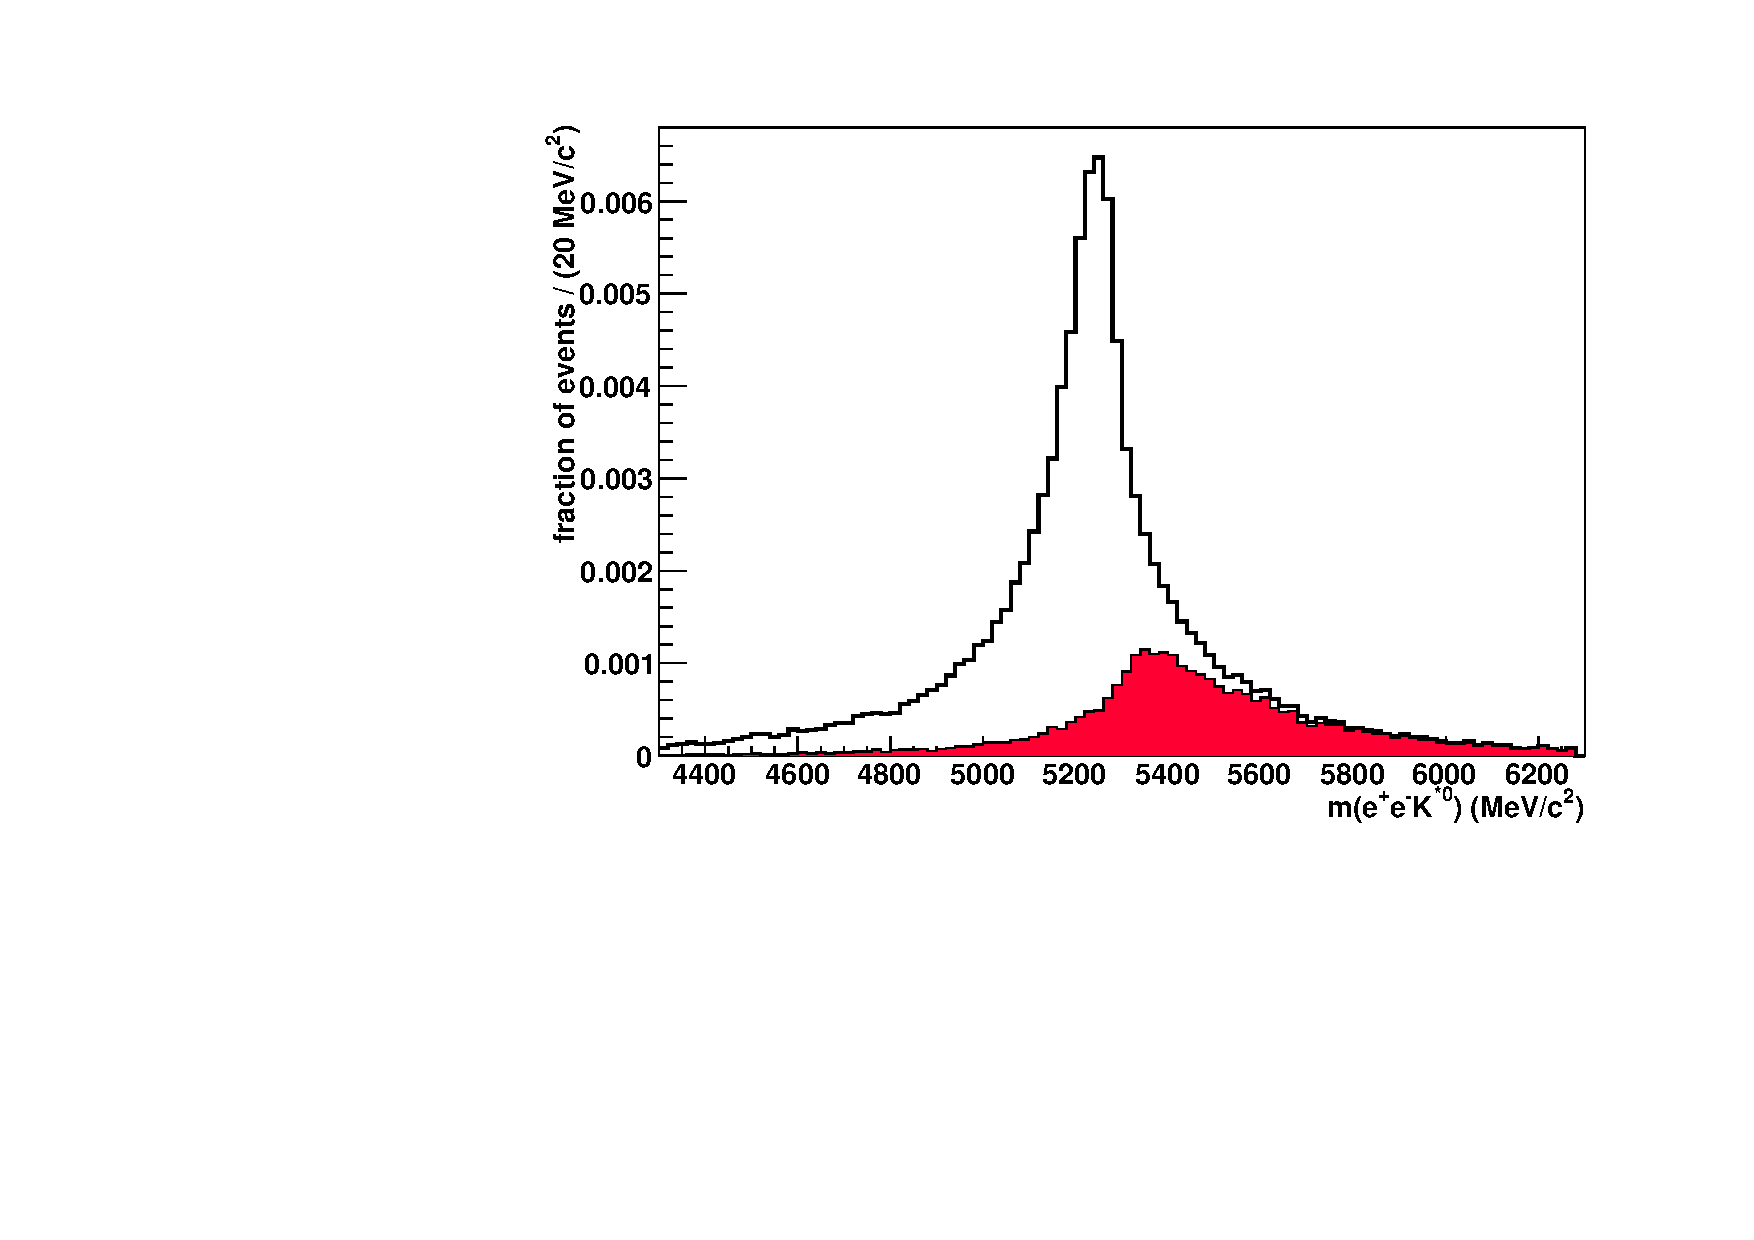
\includegraphics[width=0.49\textwidth]{MC_Bmass_dielectron_TM_nodccorrection_simplehisto.pdf}} 
  \subfigure{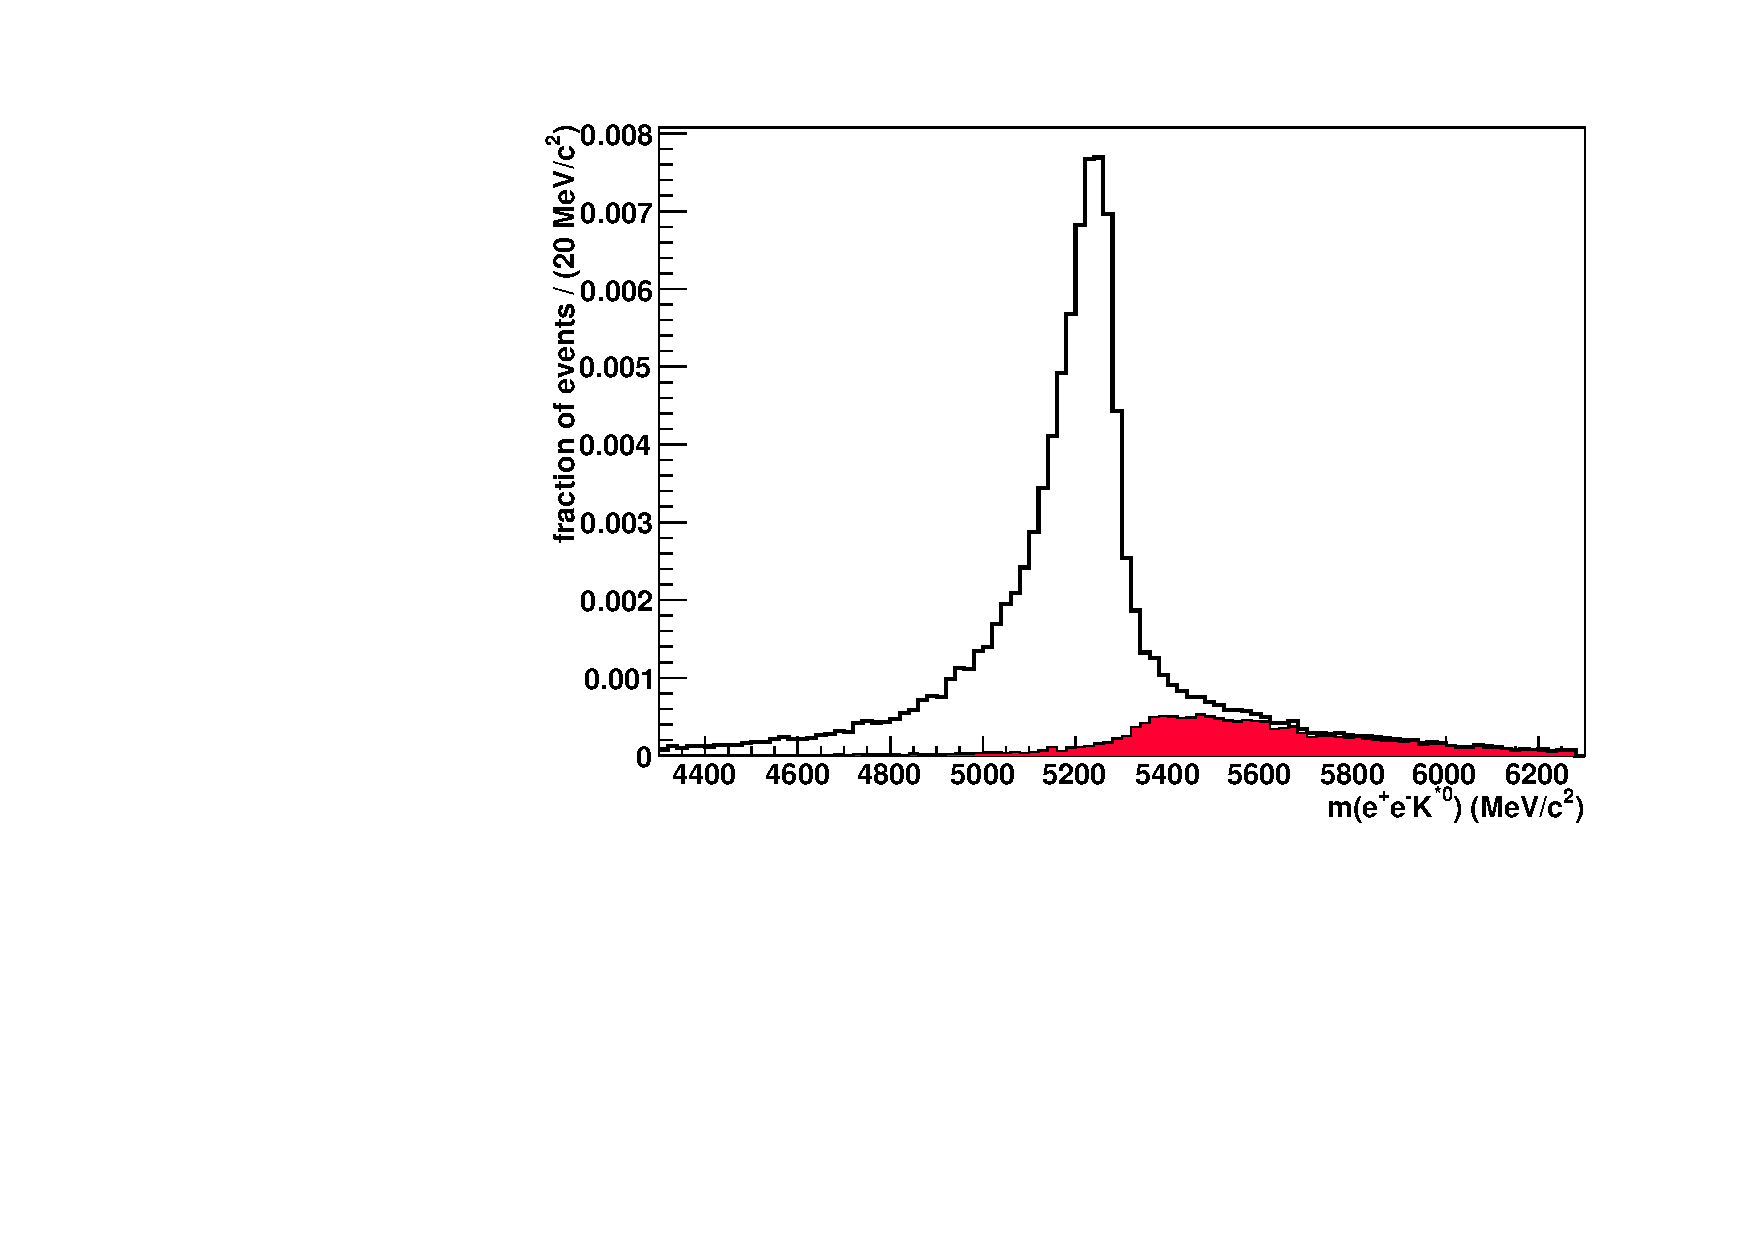
\includegraphics[width=0.49\textwidth]{MC_Bmass_dielectron_TM_nodccorrection_simplehisto_newBrem.pdf}}
  \vspace*{-1.0cm}
  \end{center}
  \caption{\textit{\Bd mass shape. The pink distribution are the events with double counting. The \Bd distribution is obtained by reconstructing \lhcb Monte Carlo with \davinci v29 (left) and \davinci v30 (right) respectively.}}
  \label{fig:oldBremAddernodcc}
\end{figure}
As can be seen from Figures \ref{fig:oldBremAddernodcc} and \ref{fig:Minveedouble counting} the amount of double counting is higher for the \davinci v29 bremsstrahlung recovery. The \lhcb Monte Carlo sample shows that double counting events account for 27 \% of all the signal events in \davinci 29 while it's only about 14\% of the signal events for \davinci v30. \\



\subsubsection{The double counting correction}
\label{sub:doublecountingcorrection}
In the course of the analysis four different methods to encounter the problem of double counting have been developed and tested:
\begin{compactenum}[a)]
\item The energy of the double counted photon candidate is assigned to the lepton with lower energy.
\item The energy of the double counted photon candidate is assigned to the lepton with higher energy.
\item The energy of the double counted photon candidate is assigned to a randomly chosen lepton. 
\item The energy of the double counted photon candidate is equally divided between the two leptons.
\end{compactenum}
After assigning the bremsstrahlung photon's energy, the four-momenta of the leptons is recalculated. From these new lepton four-momenta and the original four-momenta of the Kaon and the Pion the \Bd mass is recalculated.\\
The recalculated \Bd mass distributions for the four different methods applied to the \BdKstee \lhcb Monte Carlo sample made with the \davinci v29 are shown in Figure \ref{fig:double countingcorrection}. \\
While the first three methods yield extremely similar results, the fourth method does not reproduce the \Bd mass shape correctly. For further analysis the third method of encountering double counting is chosen. Assigning of the bremsstrahlung photon's energy to one randomly chosen electron does not undergo the risk of biasing any energy distribution and yields the most accurate \Bd mass reconstruction of the four tested algorithms.\\
\begin{figure}[ht]
\vspace*{-0.4cm}
  \begin{center}
    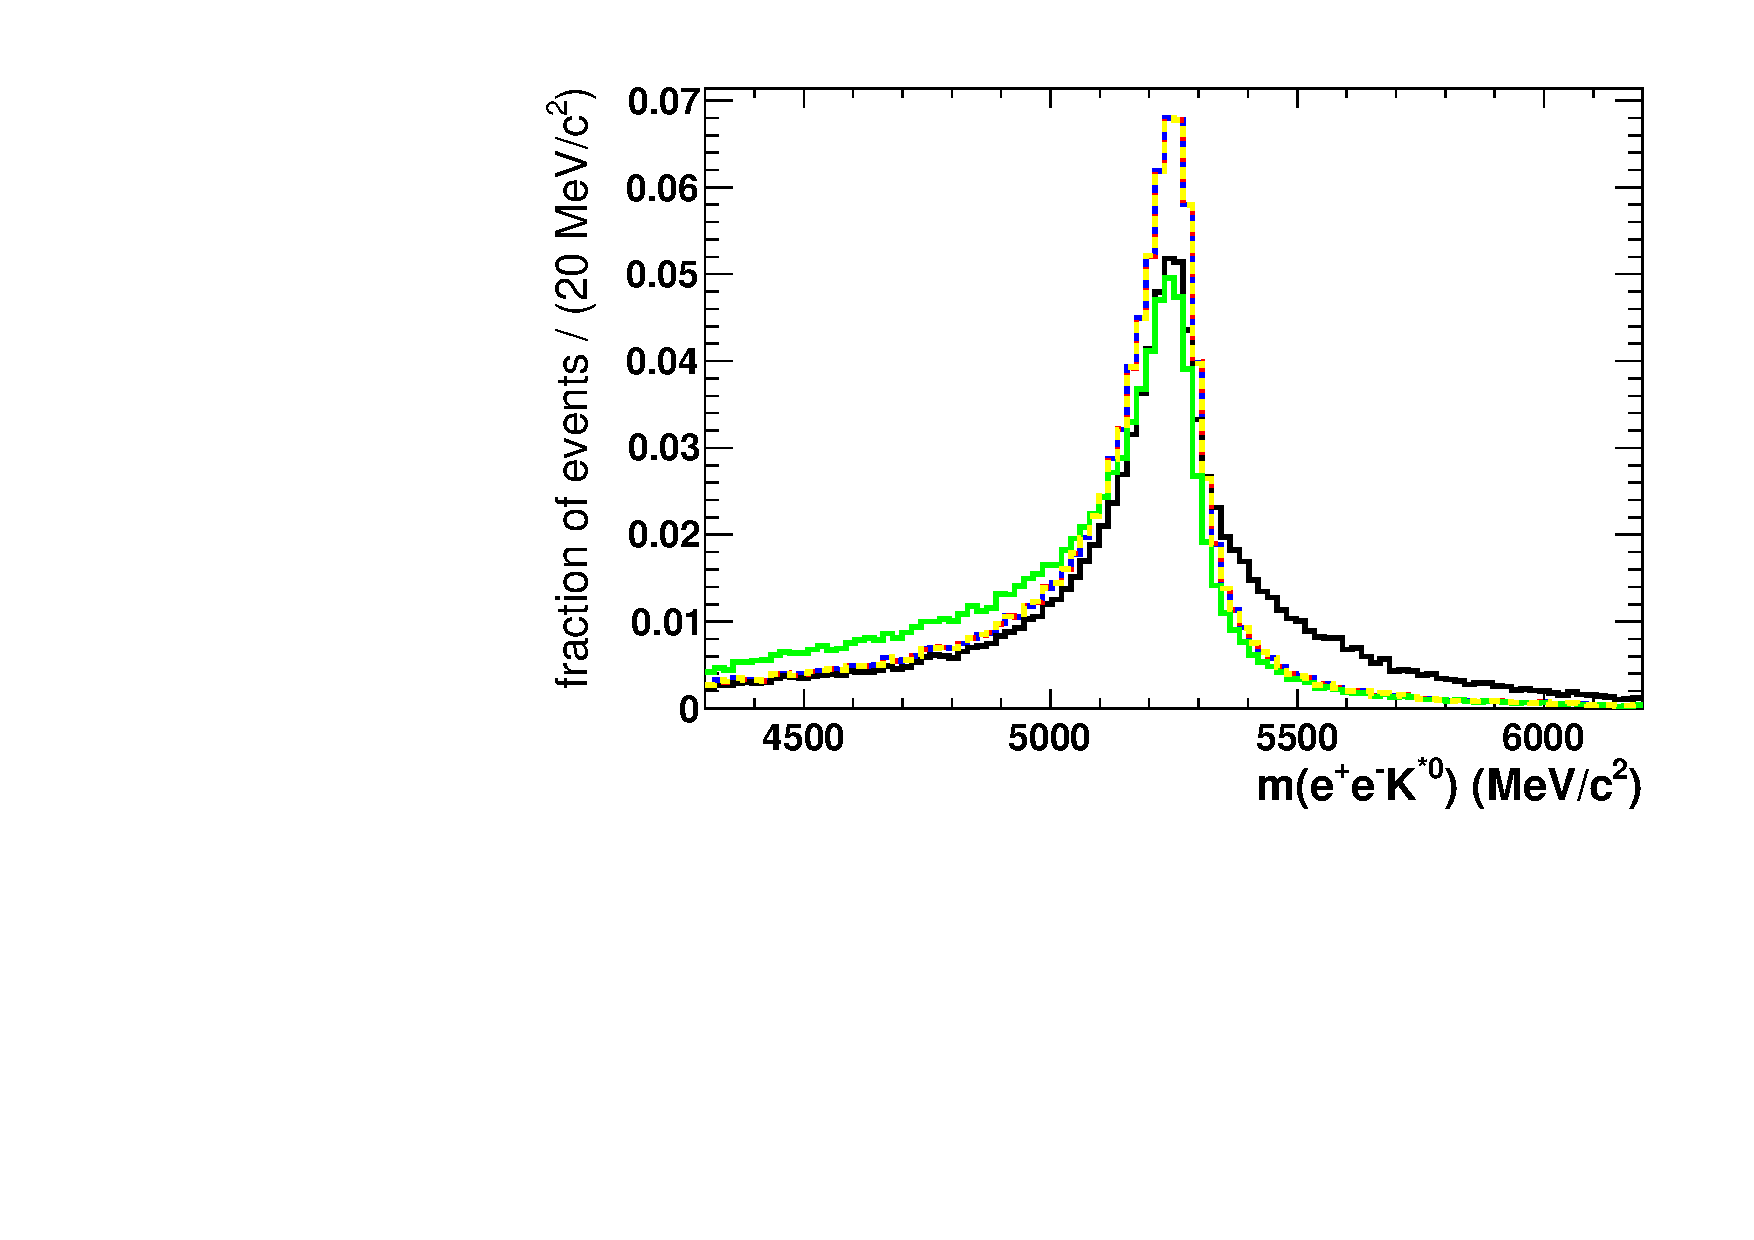
\includegraphics[scale=0.6]{minvB_nodccorrection.pdf}
  \vspace*{-1.0cm}
  \end{center}
  \caption{\textit{\Bd mass shapes for different algorithms of double counting correction. Black: no double counting correction; red: a); yellow: b); blue: c); green: d). }}
  \label{fig:double countingcorrection}
\end{figure}
\\

\subsection{Comparison of bremsstrahlung recovery algorithms}
The two bremsstrahlung recovery tools are applied to the \BdKstee \lhcb Monte Carlo, together with the double counting correction developed in the previous section. Additionally the selection developed for the 2011 dataset \cite{michellesthesis} is applied to the samples to estimate the effects on the final dataset.\\
To quantify the quality of the reconstruction tools a double Crystal-Ball distribution \cite{crystal} (for more details see Section \ref{sec:pdfs}) is fitted to the \Bd mass shape. The two Crystal-Ball distributions share the same $\mu_{\B}$, $\alpha$ and $n$. A weighted width $\sigma^w$ is calculated from the width $\sigma_1$ and $\sigma_2$ from the two Crystal-Ball distributions, where $f$ denotes the relative contribution from the first Crystal-Ball distribution.
\begin{equation}
\sigma^w = f \sigma_1 + (1- f) \sigma_2
\end{equation}

The two resulting distributions can be seen in Figure \ref{fig:comparebrems}. The resulting weighted resolutions are listed in Table \ref{tab:sigmaw}.

\begin{figure}[!h]
\vspace*{-0.cm}
  \begin{center}
  \subfigure{\label{fig:oldBremAdder}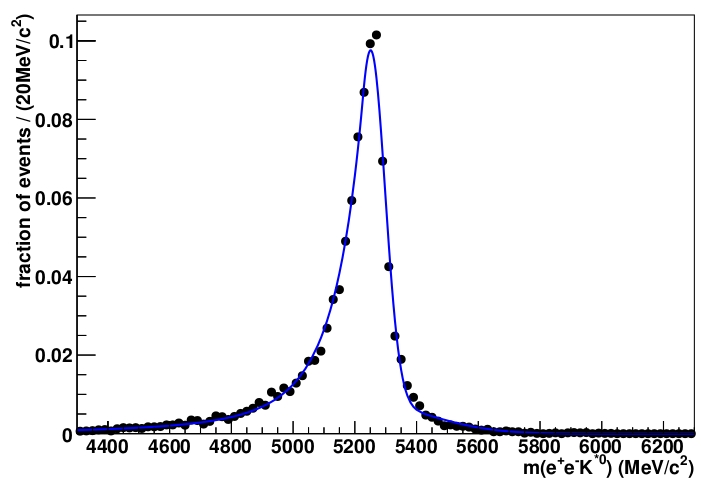
\includegraphics[width=0.49\textwidth]{oldBrem_crystalfit.jpg}}
  \subfigure{\label{fig:newBremAdder}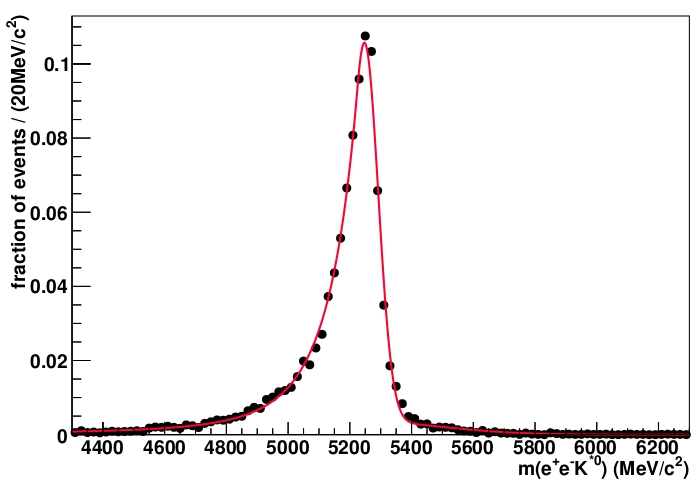
\includegraphics[width=0.48\textwidth]{newBrem_crystalfit.jpg}} 
  \vspace*{-1.0cm}
  \end{center}
  \caption{\textit{\Bd mass distribution obtained from \lhcb Monte Carlo with \davinci v29 (left) and \davinci v30 (right) and the double counting correction.}}
  \label{fig:comparebrems}
\end{figure}

\begin{table}[!h]
\begin{center}
\begin{tabular}{c|c|c|c|c}
& $\sigma_1$ & $\sigma_2$ & $f$ & $\sigma^w$ \\
\hline
\davinci v29 &  47 \mevcc & 199 \mevcc & 0.76 & 83 \mevcc \\
\hline
\davinci v30 & 45 \mevcc & 251 \mevcc & 0.86 & 74 \mevcc \\
\end{tabular}
\end{center}
\vspace*{-0.5cm}
\caption{\textit{Relevant results of the fit of a double Crystal-Ball distribution to the \BdKstee \lhcb Monte Carlo reconstructed with \davinci v29 and \davinci v30 and the double counting correction. $\sigma^w$ denotes the weighted width.}}
\label{tab:sigmaw}
\end{table}
By using the bremsstrahlung reconstruction in \davinci v30, the resolution of the \Bd mass can by increased about $13\ $\%. \\


\subsection{Effect of bremsstrahlung radiation and reconstruction on the \Bd mass shape}
Despite the implementation of the bremsstrahlung recovery tools, bremsstrahlung radiation affects the reconstructed \Bd mass shape. This can be seen in Figure \ref{fig:electronAndMuonBMass} where the reconstructed \Bd from \BdKstee is shown in direct comparison to the distribution of the \Bd mass from \BdKstmumu.\\
One effect is the large tail of the \Bd mass distribution from \BdKstee towards low \Bd masses. This tail originates from events whose bremsstrahlung photons could not be recuperated, resulting in a 
measured electron energy smaller than the initial electron energy $E^{measured}_{\epm} = (1 - E_{bs}) E^0_{\epm}$. \\
The second effect is the downgraded mass resolution which stems from the great uncertainty on the energy measurement of the calorimeter. In \lhcb the energy measurement of charged particle is performed by using combined information from the tracking system and the particle identification system. The tracking system determines the momentum of the charged particle $p_T^{track}$ with a relative accuracy of about $0.5 $\%. The particle identification system determines the identity of the particle which fixes the invariant mass of the particle track to the PDG value $m^{PDG}$. The particle's energy $E$ is then calculated from the combination of the measured momentum and the PDG \cite{pdg} \footnote{Particle Data Group.} mass.
\begin{equation}
E = \sqrt{p^2_{track} + m^2_{PDG}}
\end{equation}
The relative energy resolution is thus also of the order of $0.5 $\%.\\
For neutral particles however, the energy measurement has to be performed by the calorimeter. Since the relative energy resolution of the calorimeter is  
\begin{equation}
\frac{\sigma_E}{E} = \frac{10 \%}{\sqrt{E}} \oplus 1 \%
\end{equation}
the energy resolution of neutral particles is much worse than the energy resolution of charged particles.\\
Electrons, like muons, are charged particles and their tracks' transverse momenta $p_T^{track}(\epm)$ could be determined with an average relative accuracy of $0.5$\%. The energy of the bremsstrahlung photons however, has to be determined by the \ecal. The increase in uncertainty on the electron energy will propagate to the measured \Bd mass. \\
Figure \ref{fig:electronAndMuonBMass} shows the comparison between the \Bd mass shape of the \BdKstee and the \BdKstmumu.
\begin{figure}[ht]
  \begin{center}
  \subfigure{
  	\label{fig:eeKstar}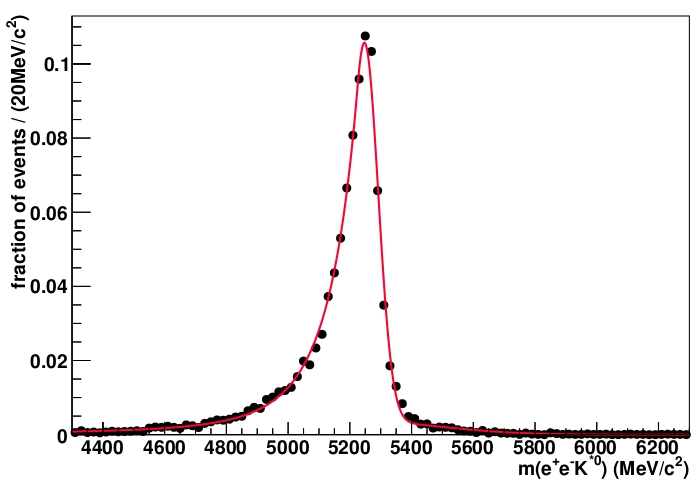
\includegraphics[width=0.49\textwidth]{newBrem_crystalfit.jpg}}
  \subfigure{\label{fig:mumuKstar}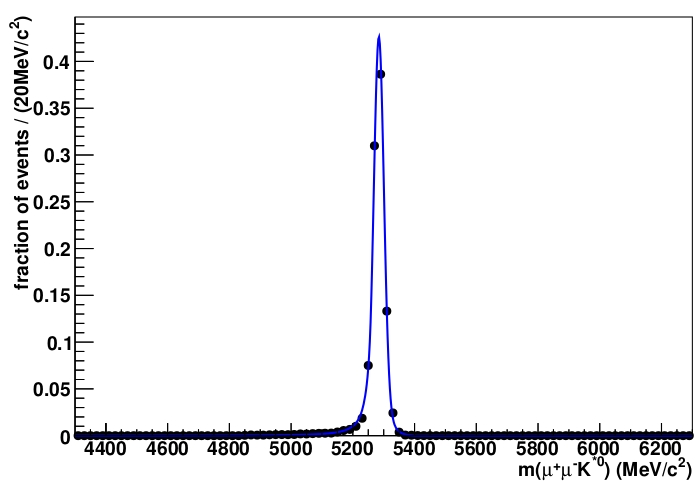
\includegraphics[width=0.49\textwidth]{MC_Bmass_mumuKstar_TM.jpg}} 
  \vspace*{-1.0cm}
  \end{center}
  \caption{\textit{Comparison of the \Bd mass distribution from \BdKstee (left) and \BdKstmumu (right) reconstructed from \lhcb Monte Carlo samples. The distribution from  \BdKstee is much wider and shows a tail at low \Bd masses, while the distribution for \BdKstmumu is just a very narrow peak.}}
  \label{fig:electronAndMuonBMass}
\end{figure}


\section{$M_{inv}(\epem)$ reconstruction}
\label{sec:DiElectronMaker}
The correct reconstruction of the invariant mass of the $e^+ e^-$ pair in the \BdKstee decay is crucial for the measurement of the various amplitudes contributing to the decay since they depend on the $M_{inv}(\epem)$ (see Chapter \ref{chapter1}).\\
In \davinci v31 a new tool designed to make opposite and same sign electron pairs was introduced. This tool -- the so-called \dielectronmaker  \ -- was specially developed to reconstruct low invariant mass $e^+ e^-$ pairs, such as electrons and positrons from converted photon or light resonances.\\
\\
While usually electron pairs are being made by combining two reconstructed electrons, the \dielectronmaker accesses the raw detector information for the electron and the positron candidates directly. Based on the hits associated to the two candidates' tracks the \dielectronmaker creates a \textit{DiElectron object} first and only then computes the properties of the individual electron and positron respectively. The \dielectronmaker chooses tracks with a $p_T$ greater than $100 \mevc$ as electron candidates. It composes the \textit{DiElectron object} from opposite sign electron pair tracks and then applies the bremsstrahlung recovery tool from \davinci v30. In the case of double counting within one \textit{DiElectron object} the four-momentum of the photon candidate is added to one randomly chosen electron, similarly to the double counting correction in Section \ref{sub:doublecountingcorrection}. Then the four-momenta of the \textit{DiElectron object} and the electron and the positron are calculated and a $p_T(e^+ e^-)$ cut greater than $500 \mevc$ is applied.
From this \textit{DiElectron object} the rest of the event reconstruction follows as usual.\\
\\
The \dielectronmaker was created to increase the efficiency of reconstruction for events with low invariant mass $e^+ e^-$ pairs and also yields a more precise reconstruction of the \Bd mass as can be seen on the Monte Carlo sample in Figure \ref{fig:diElectron}. Additionally the selection developed for the 2011 dataset \cite{michellesthesis} is applied to the sample to estimate the effects on the final dataset. The results of the fit of the double Crystal-Ball distribution to the sample are listed in Table \ref{tab:disigmaw}, showing that the use of this new tool decreases the $\sigma^w$ even further than the reconstruction by \davinci v30  yielding a reduction of $27 \ $\% with respect to the reconstruction implemented in \davinci v29.
\begin{figure}[ht]
  \begin{center}
  \subfigure{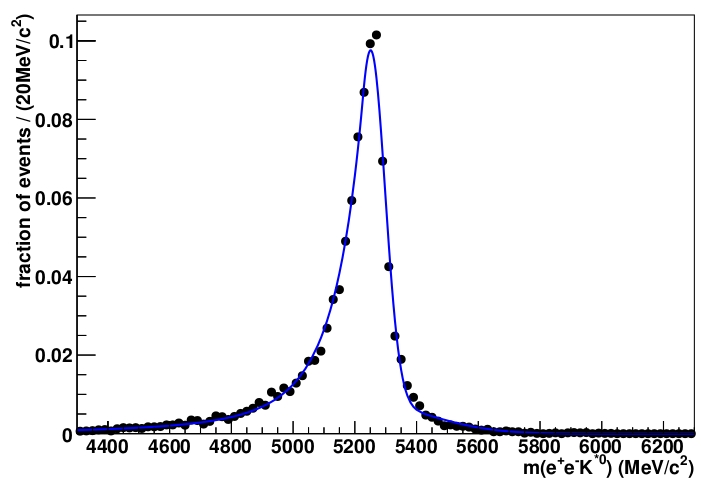
\includegraphics[width=0.49\textwidth]{oldBrem_crystalfit.jpg}}
  \subfigure{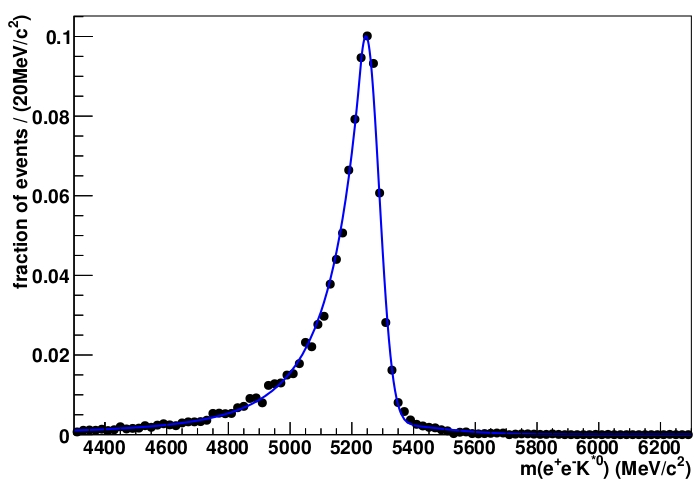
\includegraphics[width=0.49\textwidth]{diElectron_crystalfit.jpg}} 
  \end{center}
  \caption{\textit{\Bd mass distribution obtained from \lhcb Monte Carlo with \davinci v29 and double counting correction (left) and the \dielectronmaker of \davinci v31 (right).}}
  \label{fig:diElectron}
\end{figure}

\begin{table}[hc]
\begin{center}
\begin{tabular}{c|c|c|c|c}
& $\sigma_1$ & $\sigma_2$ & $f$ & $\sigma^w$ \\
\hline
\davinci v29 &  47 \mevcc & 199 \mevcc & 0.76 & 83 \mevcc \\
\hline
\davinci v31 & 54 \mevcc &  306 \mevcc & 0.91 &  77 \mevcc \\
\end{tabular}
\end{center}
\vspace*{-0.5cm}
\caption{\textit{Relevant results of the fit of a double Crystal-Ball distribution to the \BdKstee \lhcb Monte Carlo reconstructed with \davinci v29 and the double counting correction and \davinci v31. $\sigma^w$ denotes the weighted width.}}
\label{tab:disigmaw}
\end{table}

Figure \ref{fig:deltaee} shows the resolution of the dilepton invariant mass obtained from \BdKstee Monte Carlo for a dilepton invariant mass between 20\mevcc and 30\mevcc and 30\mevcc and 50\mevcc respectively. The resolutions are computed for the Monte Carlo sample that was processed with each  \davinci v29 and \davinci v31.\\
The plots show that the histograms from \davinci v31 are better centred and their Root Mean Square (RMS) is reduced by 20\% to 30\%. The first effect originates from the newer Bremsstrahlung recovery algorithm that is implemented in the \dielectronmaker. This recovery algorithm identifies more bremsstrahlung photons than the one in \davinci v29 and adds them to their emitting electron. The use of the \dielectronmaker reduces the RMS of the histograms with respect to those made by \davinci v29 because of the intermediate step of computing the \textit{DiElectron object}.
\begin{figure}[!h]
\vspace*{-0.cm}
  \begin{center}
    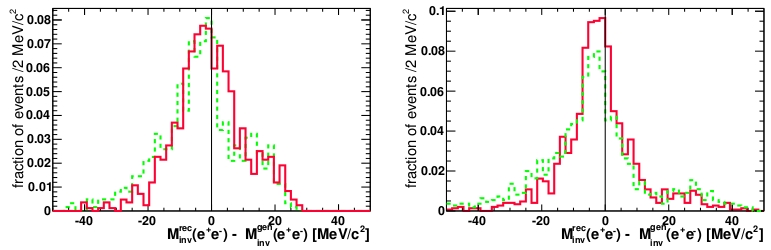
\includegraphics[scale=0.6]{deltaee.jpg}
  \vspace*{-0.5cm}
  \end{center}
  \caption{\textit{Resolution of the dilepton invariant mass obtained from the \BdKstee Monte Carlo. \textbf{Left:} The histograms for the region of 20\mevcc < $M^{gen}_{inv}(\epem)$ < 30\mevcc. \textbf{Right:} The histograms for the region of 30\mevcc < $M^{gen}_{inv}(\epem)$ < 50\mevcc. The green histogram represents the resolution of the sample processed with \davinci v29, the pink histogram represents the resolution of the sample processed with \davinci v31.}}
  \label{fig:deltaee}
\end{figure}
\\
\vspace*{1.cm}
\section{Comparison of reconstruction efficiencies}
To evaluate the performance of $M_{inv}(\epem)$ reconstruction the three reconstruction tools implemented in \davinci v29, \davinci 30 and \davinci v31 are applied to the \BdKstee \lhcb Monte Carlo respectively. After this, the double counting correction algorithm is executed on the first two samples and the selection developed for the 2011 dataset \cite{michellesthesis} \cite{paper} is applied to all three samples to estimate the effects on the final datasets.\\
Figure \ref{fig:eff_diElectron} shows the overall efficiency for reconstruction and selection of the three samples in dependency of the true -- that is generated -- invariant \epem mass $M^{gen}_{inv}(\epem)$. Note that there is a cut on the reconstructed invariant \epem mass $M^{reco}_{inv}(\epem)>30 \mevcc$\footnote{The selection developed for the 2011 dataset \cite{michellesthesis} \cite{paper} includes a tighter cut on the invariant dilepton mass than the selection developed in the course of this master's thesis}.\\
Figure \ref{fig:eff_diElectron} shows that the use of the \dielectronmaker yields the most accurate results and the highest reconstruction efficiency, especially in the region of highest interest between $30 \mevcc$ and $65 \mevcc$. The amount of reconstructed events with a generated invariant mass below $30 \mevcc$ is zero up to almost $15 \mevcc$ and then smoothly increases due to multiple scattering.\\
Above $65 \mevcc$ the efficiencies for all three reconstruction algorithms converge to the same value and remain independent of the generated invariant \epem mass.\newpage
\begin{figure}[!h]
  \begin{center}
    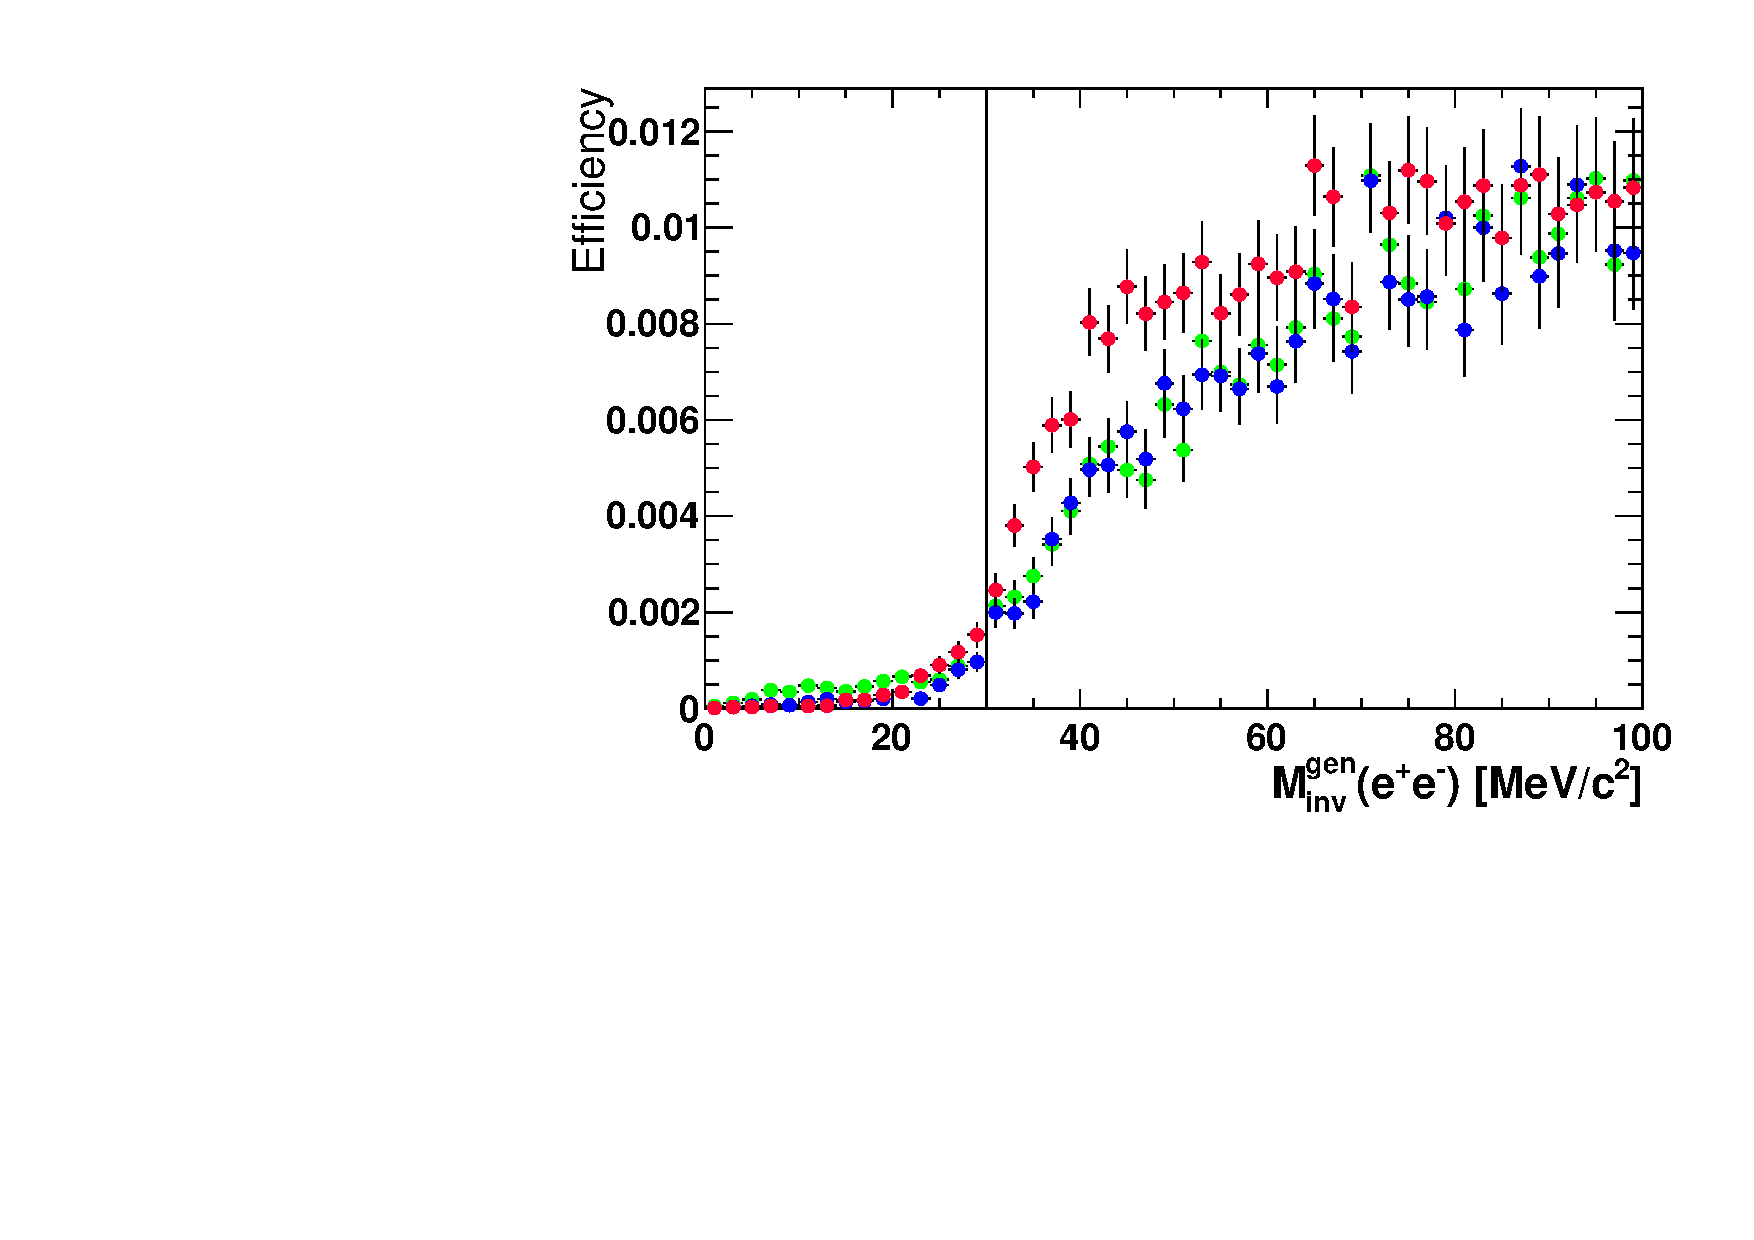
\includegraphics[scale=0.6]{eff_diElectron.pdf}
  \vspace*{-0.5cm}
  \end{center}
  \caption{\textit{Absolute event reconstruction and selection efficiency depending on the generated $M^{gen}_{inv}(\epem)$. Obtained from \BdKstee Monte Carlo by comparing the $M^{gen}_{inv}(\epem)$ at generator level with the $M^{rec}_{inv}(\epem)$ distribution after reconstruction and selection. Green: \davinci v29, blue: \davinci v30, pink: \davinci v30 with \dielectronmaker .}}
  \label{fig:eff_diElectron}
\end{figure}
\vspace*{10cm}


%%%%%%%%%%%%%%%%%%%%%%%%%%%%%%%%%%%%%%%%%%%%%%%%%%%%%%%%%%%%%%%%%%%%%%%%%%%%%%%%%%%%%%%%%%%%%%%%%%%%%%%%%%%%
%Events with double counting were identified by comparing the energy of the Bremsstrahlung photon. If this energy was non zero and the same for the photon coming %from the electron and from the positron within $5 \mev$, the event was considers to be a double counting event.

%To compare the performance of the two n-tuples of \lhcb \BdKstee Monte Carlo are created with the different bremsstrahlung recovery algorithms respectively. Then %the double counting correction is applied to both n-tuples.\\

%\subsection{DaVinci v29r1p1 BremAdder}
%\label{sub:oldBrem}
%As a first step a NTuple was created using DaVinci v29r1p1 and its standard Bremsstrahlung recovery tool. This BremAdder matches photons to the electrons by lineraly extrapolating the
%electron track from its last state before the TT to the calorimeter. If the $\chi_{brem}^2$ of the extrapolated track and the photon position in the calorimeter is less than 300, this photon is
%considerd a bremsphoton and its energy is added to the electron.\\
%Complementing this BremAdder algorithm by the \textit{double counting- correction} yields the $B^0$ mass shape in \ref{fig:oldBremAdder}. The weighted sigma of this shape is $\sigma_{w} = $.\\
%\begin{figure}[ht]
%  \begin{center}
%    \includegraphics[scale=0.6]{figs/Bmass_oldBremdcc.pdf}
%  \vspace*{-1.0cm}
%  \end{center}
%  \caption{$B^0$ mass shape for the DaVinci v29r1p1 bremsstrahlung recovery tool and double- counting correction}
%  \label{fig:oldBremAdder}
%\end{figure}
%
%\subsection{DaVinci v31r0 BremAdder}
%\label{sub:newBremAdder}
%For the second procedure a NTuple was created using DaVinci v31r0 and its standard Bremsstrahlung recovery tool. This new BremAdder is an enhanced version of the BremAdder in \ref{sub:oldBrem}. It
%uses the StdAllLoosePhotons as bremsphoton candidates by default. A photon is matched as a bremsphoton if:
%\begin{itemize}
% \item its X- position in the calorimeter is between the extrapolated X- position of the electrons first state and its extrapolated X- position from the TT within $n_x \cdot \sigma_x$ (default:
%$n_x = 2$, $\sigma_x =$ quadratic sum of photon cluster spread and track extrapolation uncertainty)
%\item its Y- position in the calorimeter matches the extrapolated Y- position from the TT within $n_y \cdot \sigma_y$ (default: $n_y = 2$, $\sigma_y =$ quadratic sum of photon
%cluster spread and track extrapolation uncertainty).
%\end{itemize}
%Complementing this BremAdder algorithm by the \textit{double counting- correction} yields the $B^0$ mass shape in \ref{fig:newBremAdder}. The weighted sigma of this shape is $\sigma_{w} = $.\\
%\begin{figure}[ht]
%  \begin{center}
%    \includegraphics[scale=0.6]{figs/Bmass_newBremdcc.pdf}
%  \vspace*{-1.0cm}
%  \end{center}
%  \caption{$B^0$ mass shape for the DaVinci v31r0 bremsstrahlung recovery tool and double- counting correction}
%  \label{fig:newBremAdder}
%\end{figure}
%
%
%\subsection{DaVinci v32 DiElectronMaker}
%\label{sub:DiElectronMaker}
%For the DaVinci v31r0 a new tool to make $e^+ e^-$ pairs has been developed (also configurable to find same sign pairs). This Tool - called \textit{DiElectronMaker} - takes the electron ProtoParticles
%and creates low invariant mass $e^+ e^-$ pairs. The DiElectronMaker uses a method of the new BremAdder (from the DaVinci v31r0) which makes it possible to avoid the double counting. In the
%case of one bremsphoton candidate matching both electrons this method adds the bremsphoton to one randomly chosen electron - 
%The DiElectronMaker then selects $e^+ e^-$ pairs that pass
%
%
%
%
%\begin{figure}[ht]
%  \begin{center}
%    \includegraphics[scale=0.6]{figs/Bmass_diElectron.pdf}
%  \vspace*{-1.0cm}
%  \end{center}
%  \caption{$B^0$ mass shape for the DaVinci v31r0 DiElectronMaker}
%  \label{fig:diElectronMaker}
%\end{figure}
%\section{Effect of bremsstrahlung radiation on the \Bd mass shape}
%The emittance of bremsstrahlung photons has two different effects on the reconstructed \Bd mass shape.\\
%The first effect can be seen on the Monte Carlo sample in Figure \ref{fig:noBremReco}. If the bremsstrahlung photons are not recuperated the measured electron energy will be smaller than the initial electron energy $E^{measured}_{\epm} = (1 - E_{bs}) E^0_{\epm}$ and this offset will propagate to the reconstructed \Bd mass. Figure \ref{fig:noBremReco} shows the \Bd mass distribution obtained without any bremsstrahlung reconstruction. The distribution has an asymmetric, non Gaussian shape with a very large radiative tail in the low \Bd mass region. Since this tail diminishes the resolution on the \Bd mass and even exceeds the reconstructed mass region, it is crucial to recuperate the emitted bremsstrahlung photons and associate them to their electrons.\\
%This bremsstrahlung recovery causes the second effect on the measured \Bd mass distribution.
%In \lhcb the energy measurement of charged particle is performed by using combined information from the tracking system and the particle identification system. The tracking system determines the momentum of the charged particle $p_T^{track}(c.p.)$ with an accuracy of about $0.5 /$\%. The particle identification system determines the identity of the particle which fixes the invariant mass of the particle track to the PDG value $m_{PDG}(c.p.)$. The particle's energy is then calculated from the combination of the measured momentum and the PDG mass $E(c.p.) = \sqrt{p^2_{track}(c.p.) + m_{PDG}(c.p.)}$. This allows for an energy resolution of the order of the momentum resolution for charged particles.\\
%For neutral particles however, the energy measurement has to be performed by the calorimeter. Since the energy resolution of the calorimeter is much worse than the momentum resolution obtained by the tracking system, the energy resolution of neutral particles is much worse than the energy resolution of charged particles.\\
%Electrons, like muons, are charged particles and their tracks' transverse momenta $p_T^{track}(\epm)$ could be determined with an accuracy up to $0.35$\%. The energy of the bremsstrahlung photons however, has to be determined by the \ecal. The increase in uncertainty on the electron energy will be propagate to the measured \Bd mass. In particular, the \Bd mass distribution reconstructed from \BdKstee will show a greater width than the \Bd mass distribution reconstructed from \BdKstmumu for example.
%Figure \ref{fig:electronAndMuonBMass} shows the comparison between the \Bd mass shape of the \BdKstee and the \BdKstmumu.
%\begin{figure}[ht]
%  \begin{center}
%  \subfigure{
%  	\label{fig:eeKstar}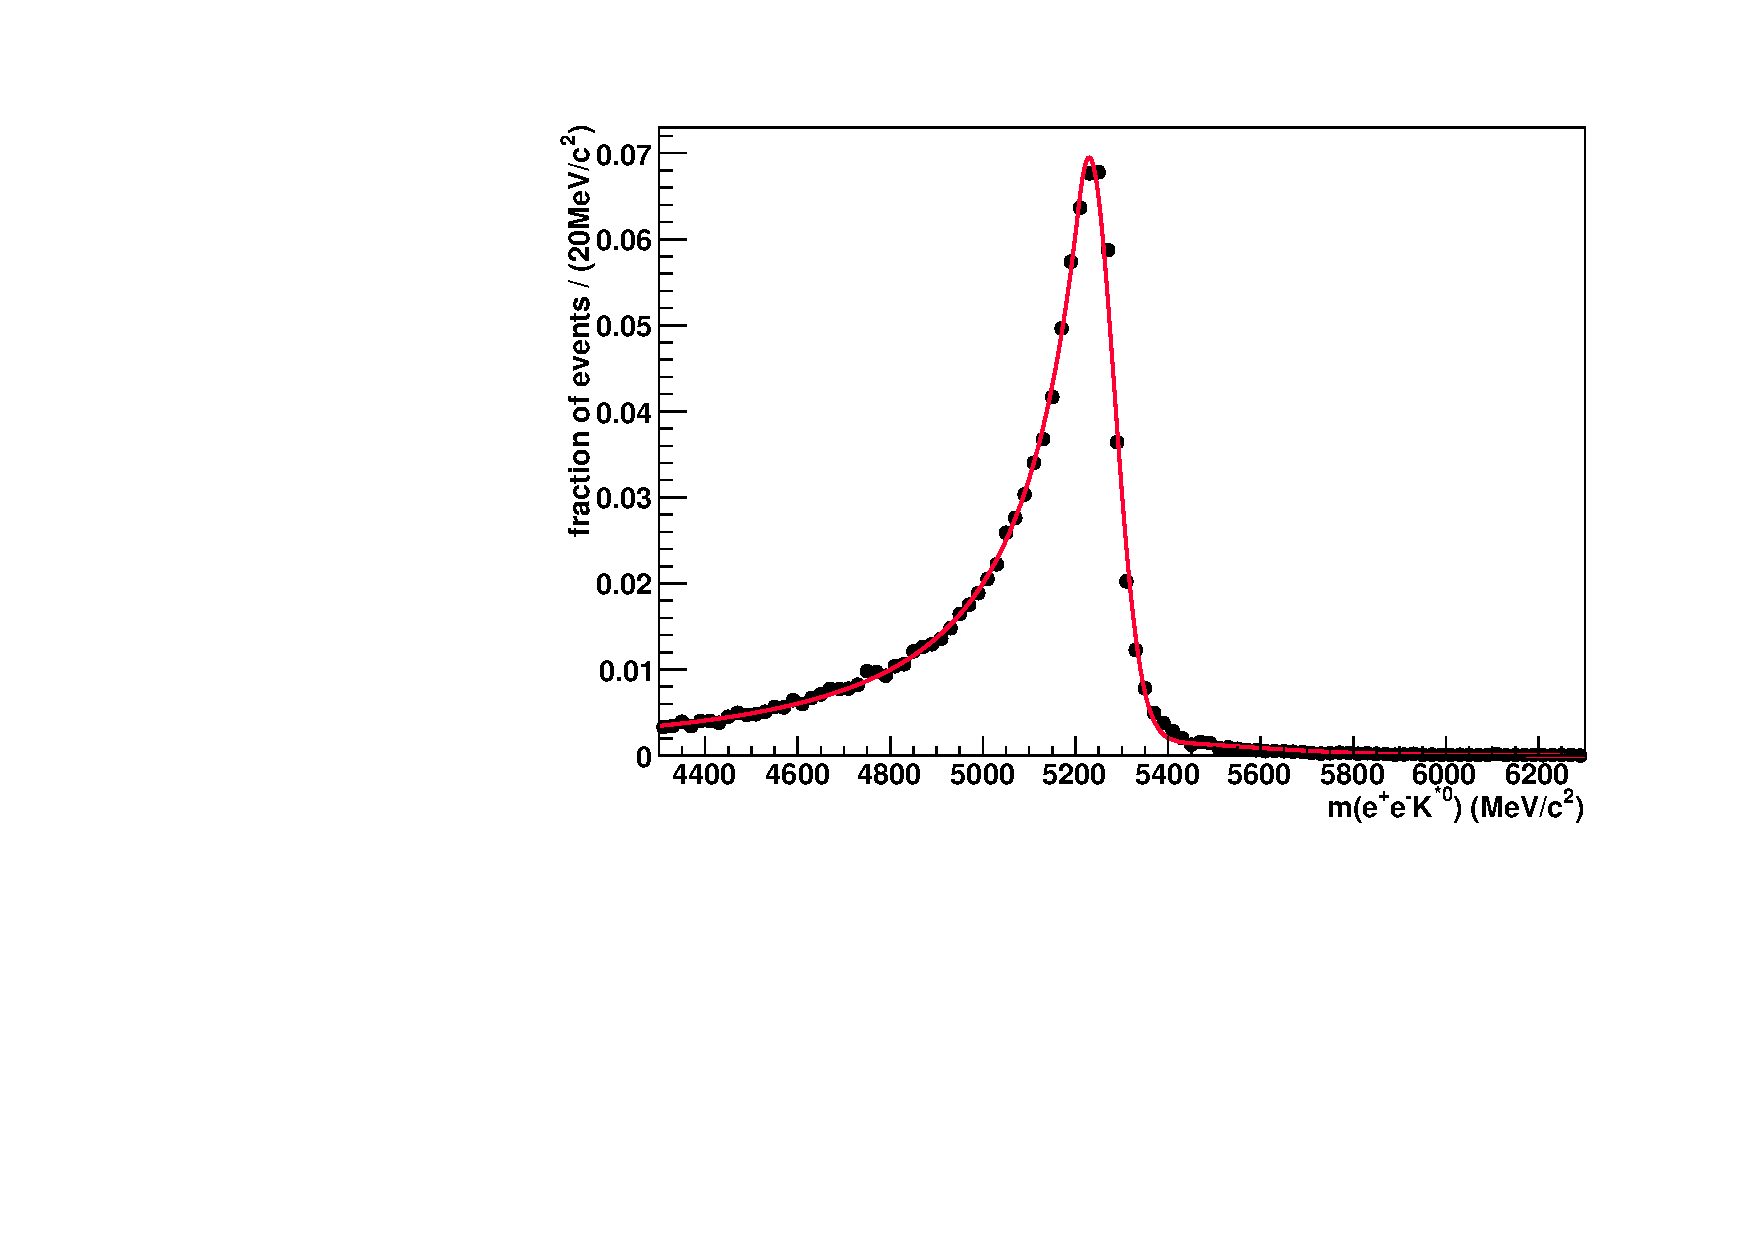
\includegraphics[width=0.49\textwidth]{MC_Bmass_dielectron_TM.pdf}}
%  \subfigure{\label{fig:mumuKstar}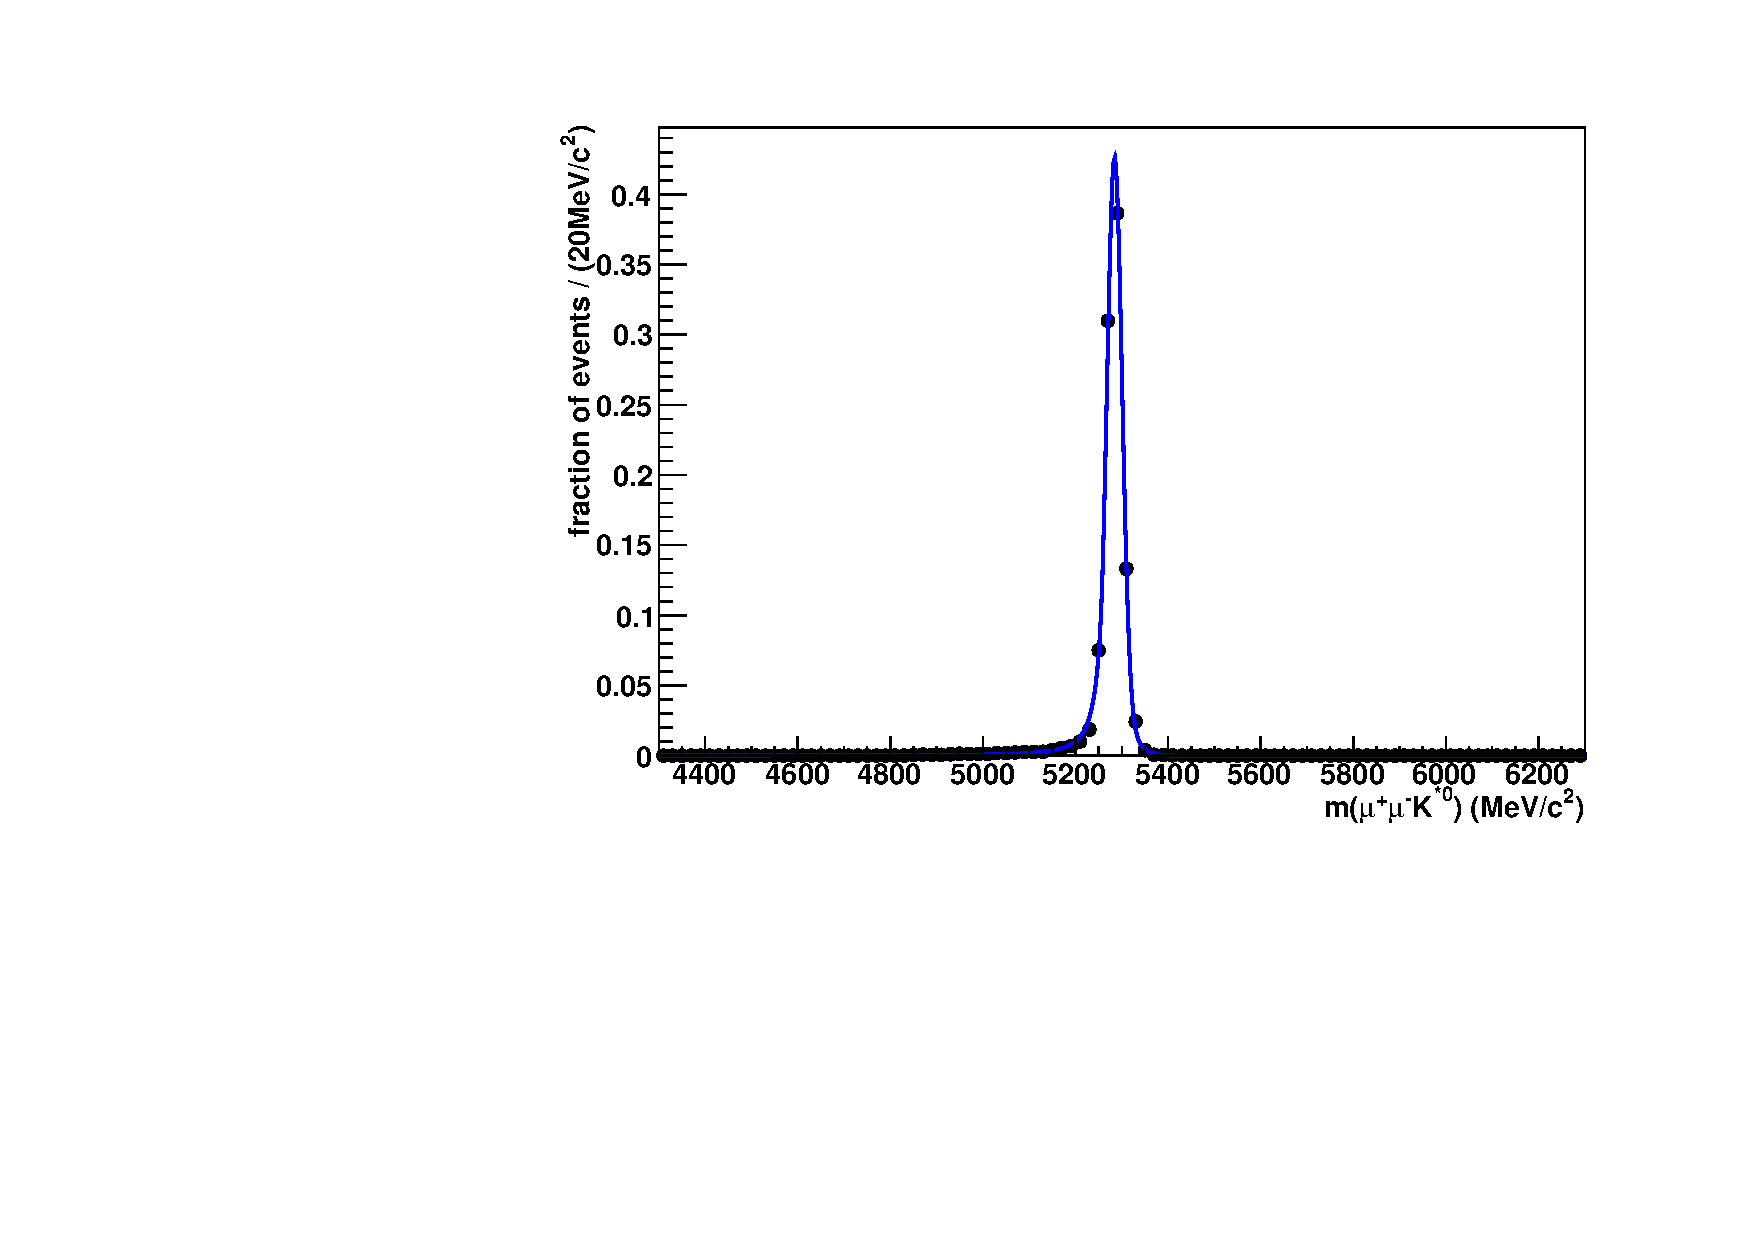
\includegraphics[width=0.49\textwidth]{MC_Bmass_mumuKstar_TM.pdf}} 
%  \vspace*{-1.0cm}
%  \end{center}
%  \caption{\textit{Comparison of the \Bd mass distribution from \BdKstee (left) and \BdKstmumu (right) reconstructed from \lhcb Monte Carlo samples.}}
%  \label{fig:electronAndMuonBMass}
%\end{figure}
